
\section{Problem formulation and methodology}
\label{sec:theory}

\subsection{The quasi-steady state (QSS) model}

The base quasi-steady state (QSS) model was first developed by \citet{Parkinson1964} for a square cross section. The equation of motion of the body  is given by 
\begin{equation}
\label{equationofmotion}
(m+m_a)\ddot{y}+c\dot{y}+ky=F_y,
\end{equation}
where the forcing term $F_y$ is given by
\begin{equation}
\label{lift equation}
F_y=\frac{1}{2}\rho U^2\mathcal{A}C_y.
\end{equation}
 
\begin{figure}
\setlength{\unitlength}{\textwidth}

  \begin{picture}(1,0.23)(0,0.74)
    
  \put(0.2,0.76){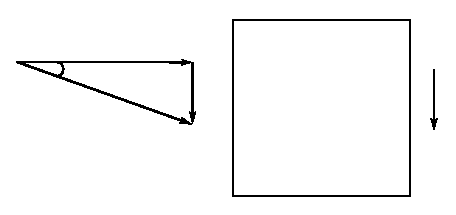
\includegraphics[width=0.5\unitlength]{../FnP/gnuplot/setup-1.eps}}         
      
      
   
 	\put(0.315,0.93){$U$}
 	\put(0.3,0.84){$U_i$}
    \put(0.42,0.88){$\dot{y}$}
    \put(0.28,0.895){ $\theta$}
    \put(0.7,0.87){\small $(+)$}
      	

 	
 	 

     

  \end{picture}

 \caption{Induced angle of attack on the square prism due to the resultant of free-stream velocity of the fluid and transverse velocity of the body.}
    \label{fig:setup_1}
\end{figure}

In the QSS model, it is assumed that the force on the body at a given instantaneous angle of attack $\theta$ (defined in figure \ref{fig:setup_1}) is the same as the mean force on a static body at the same angle of attack. The instantaneous value of $C_y$ is therefore determined by an interpolating polynomial based on the lift and drag data  for flow over a stationary body at various $\theta$. Using the relationship between $\theta$ and the instantaneous transverse velocity of the body $\dot{y}$ shown in figure \ref{fig:setup_1}, $C_y$ can be written as a function of $\dot{y}$. The order of the interpolation polynomial used to define this function has varied from study to study. For  example a $7^{th}$ order polynomial was used in \cite{Parkinson1964} and $3^{rd}$ order polynomial was used in \cite{Barrero-Gil2009}. \cite{Ng2005} concluded that using a $7^{th}$ order polynomial is sufficient and a polynomial higher than that of $7^{th}$ order doesn't provides a significantly better result. Thus a $7 ^{th}$ order interpolating polynomial is used in this present study. As a result, $C_y(\dot{y})$ is defined as
\begin{equation}
\label{cy ploynomial}
C_y(\theta)=a_1\left(\frac{\dot{y}}{U}\right)+a_3\left(\frac{\dot{y}}{U}\right)^3+a_5\left(\frac{\dot{y}}{U}\right)^5+a_7\left(\frac{\dot{y}}{U}\right)^7.
\end{equation}

%\begin{equation}
%\label{modified_equation_of_motion}
%\ddot{y}+c^*\dot{y}+k^*y=\frac{1}{2}\rho U^2A
%\end{equation}

 It is expected that vortex shedding will be well correlated along the span and provide significant forcing at low \reynoldsnumber. \citet{Joly2012} introduced  an additional sinusoidal forcing function to the hydrodynamic forcing to model this. This enables the model to provide accurate predictions even at low mass ratios where galloping excitation is suppressed or not present. In this study, the forcing due to vortex shedding in low \reynoldsnumber\ cases is incorporated using a sinusoidal forcing function $F_0\sin{\omega_{s}t}$ added to the right-hand side of equation \ref{equationofmotion}. Here, $\omega_{s}$ and $F_0$ represent the angular vortex shedding frequency and the maximum force due to shedding respectively. Thus, the final equation for the modified QSS model is

\begin{equation}
\label{final_equation_motion}
(m{+}m_a)\ddot{y}{+}c{+}\dot{y}{+}ky{=}\frac{1}{2}\rho U^2 \mathcal  {A} \Bigg(a_1\left(\frac{\dot{y}}{U}\right){+}a_3\left(\frac{\dot{y}}{U}\right)^3{+}a_5\left(\frac{\dot{y}}{U}\right)^5{+}a_7\left(\frac{\dot{y}}{U}\right)^7 \Bigg){+} F_0\sin{(\omega_s t)}.
\end{equation}

This equation could be solved using standard time integration methods. In  this study the fourth-order Runge-Kutta scheme built in to the MATLAB routine `ode45' was generally used to obtain the solutions. Some low mass ratio cases used a solver modified for stiff problems, built into the `ode15s' routine in MATLAB.

\subsection{Calculation of average power}

 The dissipated power due to the mechanical damping represents the ideal potential amount of harvested power output. Therefore, the mean power output can be given by
\begin{equation}
\label{power}
P_{mean}=\frac{1}{T}\int_{0}^{T}(c\dot{y})\dot{y} dt,
\end{equation}
where $T$ is the period of integration and $c$ is the mechanical damping constant. 

It should be noted that this quantity is equal to the work done on the body by the fluid, defined as
\begin{equation}
\label{power_alt}
P_{mean}=\frac{1}{T}\int_{0}^{T}F_y\dot{y} dt,
\end{equation}
where $F_y$ is the transverse (lift) force.

These two definitions show two important interpretions of the power with respect to any energy production device. The first shows that power will be high for situations where the damping coefficient is high, and the transverse velocity is consistently high. The second shows that power will be high for situations where the transverse force and the body velocity are in phase.
 
 \begin{figure}

  \setlength{\unitlength}{\textwidth}
  \begin{picture}(1,0.25)(0,0.8)
  
    % % %90
      \put(0.025,0.81){\includegraphics[width=0.5\unitlength]{../FnP/gnuplot/lift_curve_165.eps}}
      \put(0.495,0.81){\includegraphics[width=0.5\unitlength]{../FnP/gnuplot/lift_curve_park.eps}}
 	\put(0.02,0.93){ \large $C_y$} 	
% 	\put(0.56,1.02){ $\theta$}
 	
        \put(0.25,0.8){ $\theta$} 	
        \put(0.75,0.8){ $\theta$}
        
        \put(0.105,1.01){(a)}
        \put(0.565,1.01){(b)}
      \end{picture}

  \caption{Lift coefficient, $C_y$, as a function of incidence angle $\theta$, for a static square cross section. (a) Data from simulations at $Re=165$  (b) data from \cite{Parkinson1964} at $Re=22300$. Points ($\bullet$) are measurements from the simulations. The solid lines in both plots are 7th-order interpolating polynomial used to predict the fluid forcing for the QSS model.}
    \label{fig:lift_curves}
\end{figure}

 \begin{table}[ht]

\begin{center}
\setlength{\unitlength}{\textwidth}

\begin{tabular}{c c c c c} % centered columns (4 columns)
\hline\hline %inserts double horizontal lines
\\[0.2ex]
Case & $a_1$ & $a_3$ & $a_5$ & $a_7$ \\ [0.8ex] % inserts table 
%heading
\hline 
\\[0.8ex]% inserts single horizontal line
Re=165 & 1.3 & 125.3 & 1825.73 & 8765.3 \\[0.8ex] % inserting body of the table
Re=22300 & 2.69 & 168 & 1670 & 59900 \\ [1ex] % [1ex] adds vertical space
\hline %inserts single line
\end{tabular}

\caption{Coefficient values used in the 7th order interpolation polynomial for high ($Re=22300$) and low ($Re=165$) Reynolds numbers. These data are used as input data to calculate the RHS of Eq.\ref{final_equation_motion} throughout this study.}
 
\label{table:nonlin} % is used to refer this table in the text
\end{center}
\end{table}


 
\subsection{Parameters used} 
 
For the low \reynoldsnumber\ tests, \reynoldsnumber=165 was maintained as it was pointed out by \citet{Sheard2009} and \citet{Tong2008} that the three-dimensional transition for a square cylinder occurs at approximately \reynoldsnumber=160. $F_0$ was kept at $0.4937$ which was obtained by scaling the value used by \citet{Joly2012} with the amplitude ratios of the lift forces obtained at the different Reynolds numbers. 

The angular vortex shedding frequency $\omega_s$, was set to $0.98$ which was obtained by performing a power spectral analysis of the stationary data at $0^\circ$. Stationary $C_y$ data were obtained at different angles of attack ranging from $0^\circ$ to $16^\circ$. The average power was obtained by using Eq.\eqref{power}, and the averaging was done over no less than 20 galloping periods. Predictions of power output at \reynoldsnumber=22300 were obtained using the coefficients for curve fitting $C_y$ (Table (\ref{table:cy-coefficients})) from \citet{Parkinson1964}, in order to provide a comparison between high and low Reynolds numbers. The mass ration $m^*$ was kept at 1163 for \reynoldsnumber=22300 (Similar as \citet{Parkinson1964}) and $m^*=20$ for \reynoldsnumber=165. These parameters were used throughout this study unless otherwise specified. 

The stationary data and the fluid-structure interaction (FSI) data were obtained using a high-order spectral element routine to simulate the two-dimensional laminar flow.  Simulations involving fluid structure interaction (FSI) were used to provide additional validation of the QSS model. The inlet was placed $20D$ while the outlet situated $60D$ away from the centroid of the body. The side boundaries were placed $20D$ away from the centroid of the body where $D$ was kept as unity throughout this study. The Navier--Stokes equations were solved in an accelerated frame of reference attached to the moving body along with the body equation of motion given in equation \ref{equationofmotion}. A three-step time splitting scheme together with high-order Lagrangian polynomials were used to obtain the solution. The details of the method can be found in \cite{Thompson2006,Thompson1996a}. This code has been very well validated in a variety of fluid-structure interaction problems \citep{Leontini2007a,Griffith2011,Leontini2011,Leontini2013}.
 
 The computational domain consists of 690 quadrilateral macro elements where majority of the elements were concentrated near the square section. A freestream condition was given to the inlet, top and bottom boundaries and the normal velocity gradient was set to zero at the outlet. A convergence study was performed by changing the order of the polynomial ($p$-refinement) at $U^*=40$ and \reynoldsnumber=$165$. A $9^{th}$ order polynomial together with a time step of $\frac{\Delta tU}{D}=0.001$ was sufficient to ensure an accuracy of $2\%$ with regards to amplitude of oscillation.
